\chapter{Software-Entwurf} \label{cha:swentwurf}

\section{Blockansicht}

Im folgenden ist die Struktur (\textit{High-Level-Ansicht}) des Software-Systems in Form eines Blackbox-Diagrams dargestellt.

\begin{figure}[H]
    \centering
    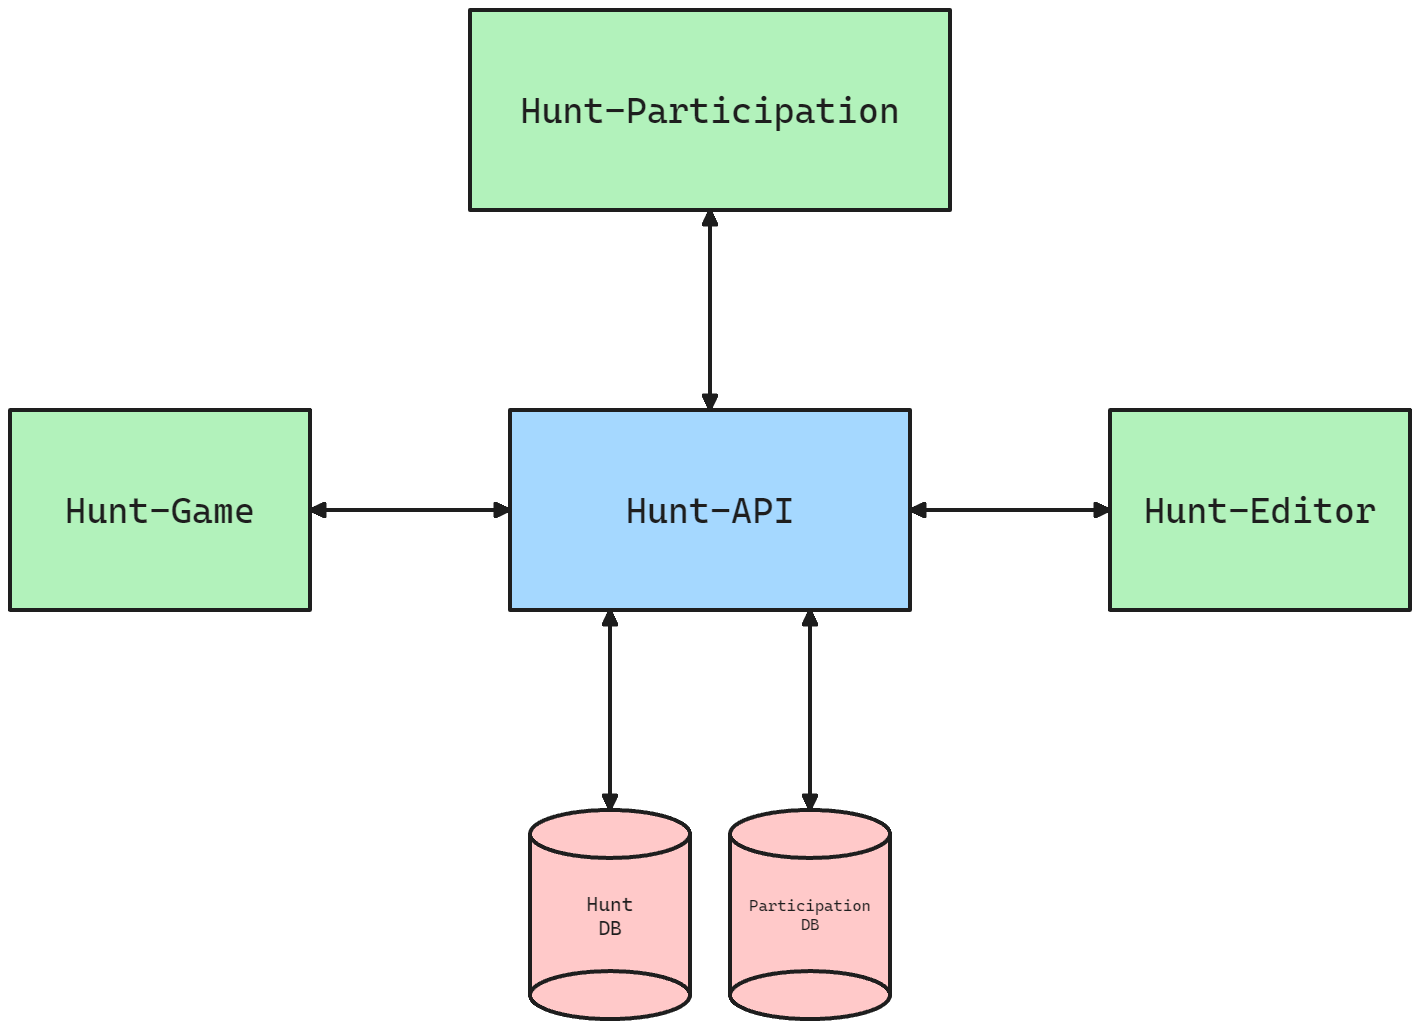
\includegraphics[width=\textwidth]{images/PrAr-Software-Entwurf-Blockansicht.png}
    \caption{Bild Systemkontext als Blackbox-Diagram}
    \label{fig:swentwurf:blackbox}
\end{figure}

Das in Abbildung \ref{fig:swentwurf:blackbox} dargestellte Blackbox-Diagramm beschreibt den Zusammenhang der unterschiedlichen Subsysteme zueinander. Die verschiedenen Aufgaben, die das System zu leisten hat, wurden als einzelne Anwendungen vorhergesehen. Diese sind in Abbildung \ref{fig:swentwurf:blackbox} grün markiert. Dies ermöglicht eine klare Trennung der verschiedenen Domänen (Erstellung, Anmeldung, Durchführung). Das Backend steht als zentrale Schnittstelle für die Bereitstellung Systemspezifischer Funktionalitäten zur Verfügung. Dieses sind in Abbildung \ref{fig:swentwurf:blackbox} blau markiert. Für die Datenpersistierung besitzt das Backend zwei Datenbank-Verbindungen. Dieses sind in Abbildung \ref{fig:swentwurf:blackbox} rot markiert.

\section{Subsysteme}

\subsection{Hunt-Api}

\subsubsection{Übersicht}

Anhand einer zentral zur Verfügung stehenden Schnittstelle \textit{Hunt-Api} können die verschiedenen Anwendungen zur Funktionalität des Systems beitragen. Die Schnittstelle bietet verschiedene Endpunkte für die Verwaltung von Schnitzeljagden, Teilnahmen und die bewältigten Aufgaben der Teilnehmer. Eine Darstellung der Hunt-API Architektur ist in Abbildung \ref{fig:swentwurf:huntapi:subsystem} näher beschrieben.

Anhand der zentral zur Verfügung stehenden Schnittstelle \textit{Hunt-Api} können die verschiedenen Anwendungen zur Funktionalität des Systems beitragen. Diese Schnittstelle bietet diverse Endpunkte für die Verwaltung von Schnitzeljagden, Teilnahmen und die bearbeiteten Aufgaben der Teilnehmer. Eine allgemeine Übersicht der Hunt-Api-Architektur ist in Abbildung \ref{fig:swentwurf:huntapi:subsystem} beschrieben.

\begin{figure}[H]
    \centering
    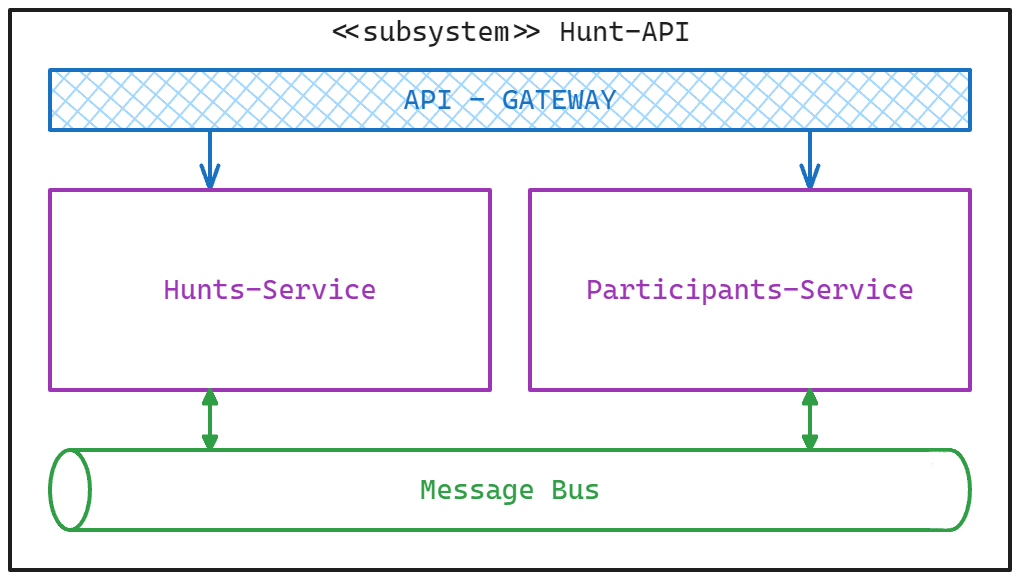
\includegraphics[width=\textwidth]{images/PrAr-Software-Entwurf-Hunt-Api-Subsystem.png}
    \caption{Bild Hunt-Api Subsystem}
    \label{fig:swentwurf:huntapi:subsystem}
\end{figure}

Als Architekturmuster wurde ein domänenorientierter Ansatz gewählt, der in Kapitel \ref{cha:grundlagen:swdesign:ddd} näher erläutert wird. Jede Domäne repräsentiert dabei einen spezifischen Teilaspekt des Gesamtsystems. Die ausgewählten Domänen, \textit{Hunts} und \textit{Participants}, sind in Abbildung \ref{fig:swentwurf:huntapi:subsystem} lila hervorgehoben unr repräsentieren den jeweiligen Dienst (Microservice).

Für die Kommunikation unterschiedlicher Dienste ist ein Message-Bus vorhergesehen, worüber eventgesteuert Nachrichten ausgestauscht werden. Dieser ist in Abbildung \ref{fig:swentwurf:huntapi:subsystem} grün hervorgehoben.

Um eine einheitliche Schnittstelle bereitzustellen, die anwendungsübergreifend genutzt werden kann, wurde ein Api-Gateway vorhergesehen. Dieses Gateway ermöglicht es, Anfragen an das Backend zu stellen und sie an die entsprechenden Dienste weiterzuleiten. Das API-Gateway ist in Abbildung \ref{fig:swentwurf:huntapi:subsystem} blau gekennzeichnet.

\subsubsection{Hunts-Service} \label{cha:swentwurf:huntsservice}

Für die Verwaltung der erstellten Schnitzeljagden eines Organisators, stellt der Hunts-Service eine Schnittstelle hierfür bereit. Abbildung \ref{fig:swentwurf:huntapi:huntservice} zeigt die Struktur des Dienstes.

\begin{figure}[H]
    \centering
    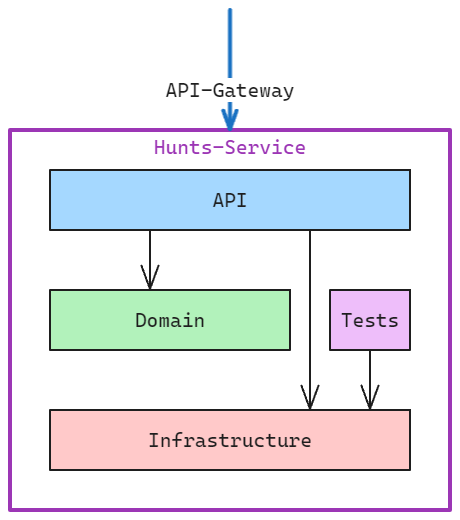
\includegraphics[width=\textwidth]{images/PrAr-Software-Entwurf-Hunt-Api-Hunt-Service.png}
    \caption{Bild Hunts Microservice}
    \label{fig:swentwurf:huntapi:huntservice}
\end{figure}

Innerhalb des Hunts-Service wurde ein schichtenorientierter Ansatz gewählt, welche Ähnlichkeiten mit der in Kapitel \ref{cha:grundlagen:swdesign:onion} beschriebenen \textit{Onion-Architecture} teilt. Jede Schicht entspricht einer horizontalen Teilung der unterschiedlichen Anwendungs-Aspekte. Für die Persistierung der Schnitzeljagden (Hunts) wurde das Repository-Pattern vorhergesehen.

Die grundlegende Funktionalität der Domäne (\textit{Hunts}, \textit{Assignments}, etc.) wird in der \textit{Domain-Schicht} zur Verfügung gestellt, welche in Abbildung \ref{fig:swentwurf:huntapi:huntservice} grün gekennzeichnet wird. Hier sind Modelle und Entities, sowie Datentypen, Enumerations und Repository-Interfaces definiert, die im System durchweg Verwendung finden. Die Domain-Schicht ist abgekapselt von Anwendungs- und Infrastrukturlogik und besitzt daher keine Abhängigkeiten zu externen Modulen.

Eine Implementierung der Repository-Interfaces wird in der \textit{Infrastruktur-Schicht} (Infrastructure) zur Verfügung gestellt, die in Abbildung \ref{fig:swentwurf:huntapi:huntservice} rot hervorgehoben wird. Diese kann zudem unabhängig von der Domänen-Logik isoliert getestet werden, wie in in Abbildung \ref{fig:swentwurf:huntapi:huntservice} lila dargestellt wird.

Die \textit{Anwendungs-Schicht} ist in Abbildung \ref{fig:swentwurf:huntapi:huntservice} blau hervorgehoben und bündelt die Funktionalität der Domain-Schicht und Infrastruktur-Schicht gemeinsam. Über eine einheitliche Schnittstelle (\textit{api/Hunt}) können Schnitzeljagden erstellt, bearbeitet, gelöscht und aufgelistet werden.

\begin{figure}[H]
    \centering
    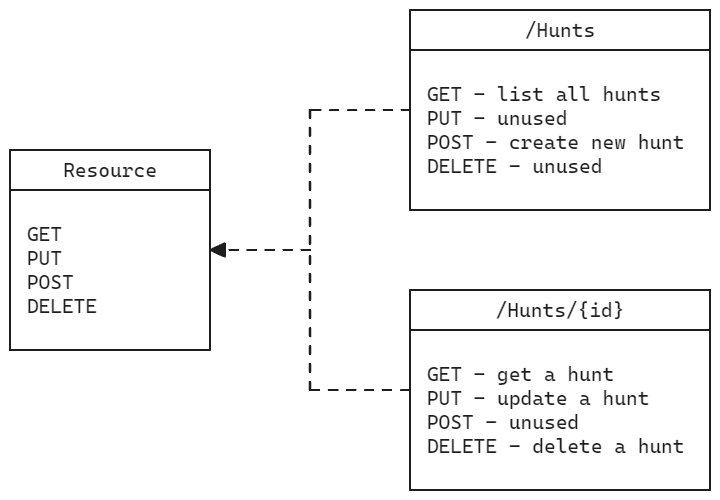
\includegraphics[width=\textwidth]{images/PrAr-Software-Entwurf-Hunt-Api-Hunt-Service-Endpoints.png}
    \caption{Skizze der Hunts Ressourcenansicht}
    \label{fig:swentwurf:huntapi:huntservice:endpoints}
\end{figure}

In Abbildung \ref{fig:swentwurf:huntapi:huntservice:endpoints} sind die unterschiedlichen Operationen auf Schnitzeljagden (\textit{Hunts}) anhand des ressourcen-orientierten Ansatz aus Kapitel \ref{cha:grundlagen:collaboration:rest} dargestellt.

\subsubsection{Participants-Service}

Damit ein Teilnehmer an einer Schnitzeljagd teilnehmen und diese auch durchführen kann, soll ihm die Anmelde- und Spielfunktionalität zur Verfügung gestellt werden. Dies wird über den Participants-Service ermöglicht. Abbildung \ref{fig:swentwurf:huntapi:participantservice} zeigt die Struktur des Dienstes.

\begin{figure}[H]
    \centering
    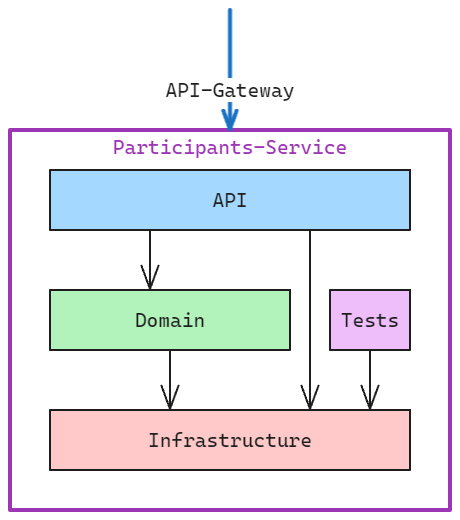
\includegraphics[width=\textwidth]{images/PrAr-Software-Entwurf-Hunt-Api-Participant-Service.png}
    \caption{Bild Participants Microservice}
    \label{fig:swentwurf:huntapi:participantservice}
\end{figure}

Der Participants-Service besitzt eine ähnliche Struktur wie der Hunts-Service aus Kapitel \ref{cha:swentwurf:huntsservice} und erfüllt die Aufgabe der Teilnahmen-Verwaltung. 

% TODO: ENDPUNKTE FÜR PARTICIPANTS UND PARTICIPATIONS


\subsection{Datenbanken-Modell}

\subsubsection{Übersicht}

% TODO: ALLGEMEINES ER DIAGRAMM

\subsubsection{Hunts-Datenbank}

% TODO: ER DIAGRAMM NUR TEIL DER HUNTS

\subsubsection{Participants-Datenbank}

% TODO: ER DIAGRAMM + REDIS CACHE STRUKTUR NUR TEIL DER PARTICIPANTS

\subsection{Hunt-Game}

\subsubsection{Entscheidung Web-App anstatt Unity}

\paragraph{Vorteile der Web-App gegenüber Unity} \mbox{}\\
Unity ist eine leistungsfähige Engine, die für die Entwicklung von 3D-Spielen und AR-Anwendungen bekannt ist. Die Implementierung von AR-Funktionen in Unity kann jedoch erheblich komplexer sein als die Entwicklung einer Web-App. Dies liegt an mehreren Faktoren:

\begin{itemize}
    \item \textbf{Entwicklungsaufwand}: Die AR-Funktionalität in Unity erfordert umfangreiche Kenntnisse in der Programmierung von AR-Erfahrungen, was die Entwicklungszeit verlängern und den Aufwand erhöhen kann. Die Handhabung von AR-spezifischen Aspekten wie der Positionierung virtueller Objekte im Raum und der Verarbeitung von Sensordaten kann zusätzliche Komplexität und Entwicklungszeit bedeuten.
    \item \textbf{Coroutines und yield}: Unity verwendet Coroutines, um asynchrone Operationen durchzuführen. Diese Mechanismen ermöglichen es, lange Operationen, wie das Warten auf eine Antwort von einem HTTP-Request, ohne das Einfrieren der gesamten Anwendung durchzuführen. Das Management von Coroutines erfordert jedoch ein spezifisches Verständnis der Unity-eigenen Programmierschnittstellen und kann zu komplexen und schwer nachvollziehbaren Code-Strukturen führen.
\end{itemize}

Das Styling und die Gestaltung von Benutzeroberflächen in Unity unterscheidet sich erheblich von der Webentwicklung. Unity verwendet ein eigenes System für die Gestaltung von UI-Elementen, das auf dem Unity Editor basiert und spezielle Komponenten wie Canvas, Panels und UI-Elemente umfasst. Für spezifische visuelle Effekte sind oft eigene Shader und Materialien erforderlich, was die Komplexität weiter erhöht. Diese benötigen tiefere Kenntnisse in der grafischen Programmierung und können den Entwicklungsprozess verlangsamen.

\textbf{Preisstruktur von Unity}\\ 
Die im September 2023 von Unity angekündigten Preisänderungen, die eine neue Laufzeitgebühr für kommerziell erfolgreiche Projekte einführten, haben die Kostenstruktur erheblich beeinflusst. Diese Gebühren sind an die Anzahl der Installationen und den jährlichen Umsatz gebunden, was insbesondere für erfolgreichere Entwickler zu einer zusätzlichen finanziellen Belastung führen kann. Die Einführung dieser Gebühren, die auch nachträglich angewendet werden können, stieß auf breite Kritik und Unsicherheit innerhalb der Entwicklergemeinschaft.

Für kleinere Projekte oder Entwickler, die nicht die Umsatz- oder Installationsschwellen erreichen, mag die neue Preisstruktur von Unity zunächst weniger relevant erscheinen. Dennoch wirft die Ungewissheit über zukünftige Preisanpassungen ernste Bedenken auf. Es ist gut möglich, dass Unity seine Preispolitik weiter verschärft, um zusätzliche Einnahmen zu erzielen. Solche Änderungen könnten die Kosten für Entwickler erheblich steigern und zusätzliche Unsicherheiten mit sich bringen. Dies könnte für das Projekt riskant sein, da dieses in der Hochschule möglichst lang eingesetzt werden sollte, ohne dafür große Lizenzkosten tragen zu müssen.

\textbf{WebAR als Alternative}\\
Eine vielversprechende Alternative zur nativen AR-Entwicklung mit Unity ist WebAR. WebAR ermöglicht AR-Erlebnisse direkt im Webbrowser ohne die Notwendigkeit einer separaten App-Installation. Dies bietet mehrere Vorteile:
\begin{itemize}
    \item \textbf{Zugänglichkeit}: WebAR ist auf jedem modernen Webbrowser verfügbar, was die Zugänglichkeit für Benutzer erleichtert und die Notwendigkeit, eine spezielle App herunterzuladen, beseitigt. Dies kann die Benutzerfreundlichkeit und die Reichweite der Anwendung erhöhen.

    \item \textbf{Einfachere Entwicklung}: WebAR nutzt Web-Technologien wie JavaScript und WebGL, die für viele Entwickler vertrauter und zugänglicher sind als die speziellen Tools und Skripte von Unity. Die Entwicklung kann daher schneller und einfacher sein, besonders wenn bereits Erfahrung mit Web-Technologien besteht.

    \item \textbf{Kosteneffizienz}: Da WebAR keine zusätzlichen Lizenzgebühren oder Laufzeitgebühren erfordert, ist es eine kostengünstigere Lösung.

\end{itemize}

\subsubsection{Übersicht}

% TODO: Architektur Unity App (?)

\subsection{Hunt-Editor}

\subsubsection{Übersicht}

\begin{figure}[H]
  \centering
  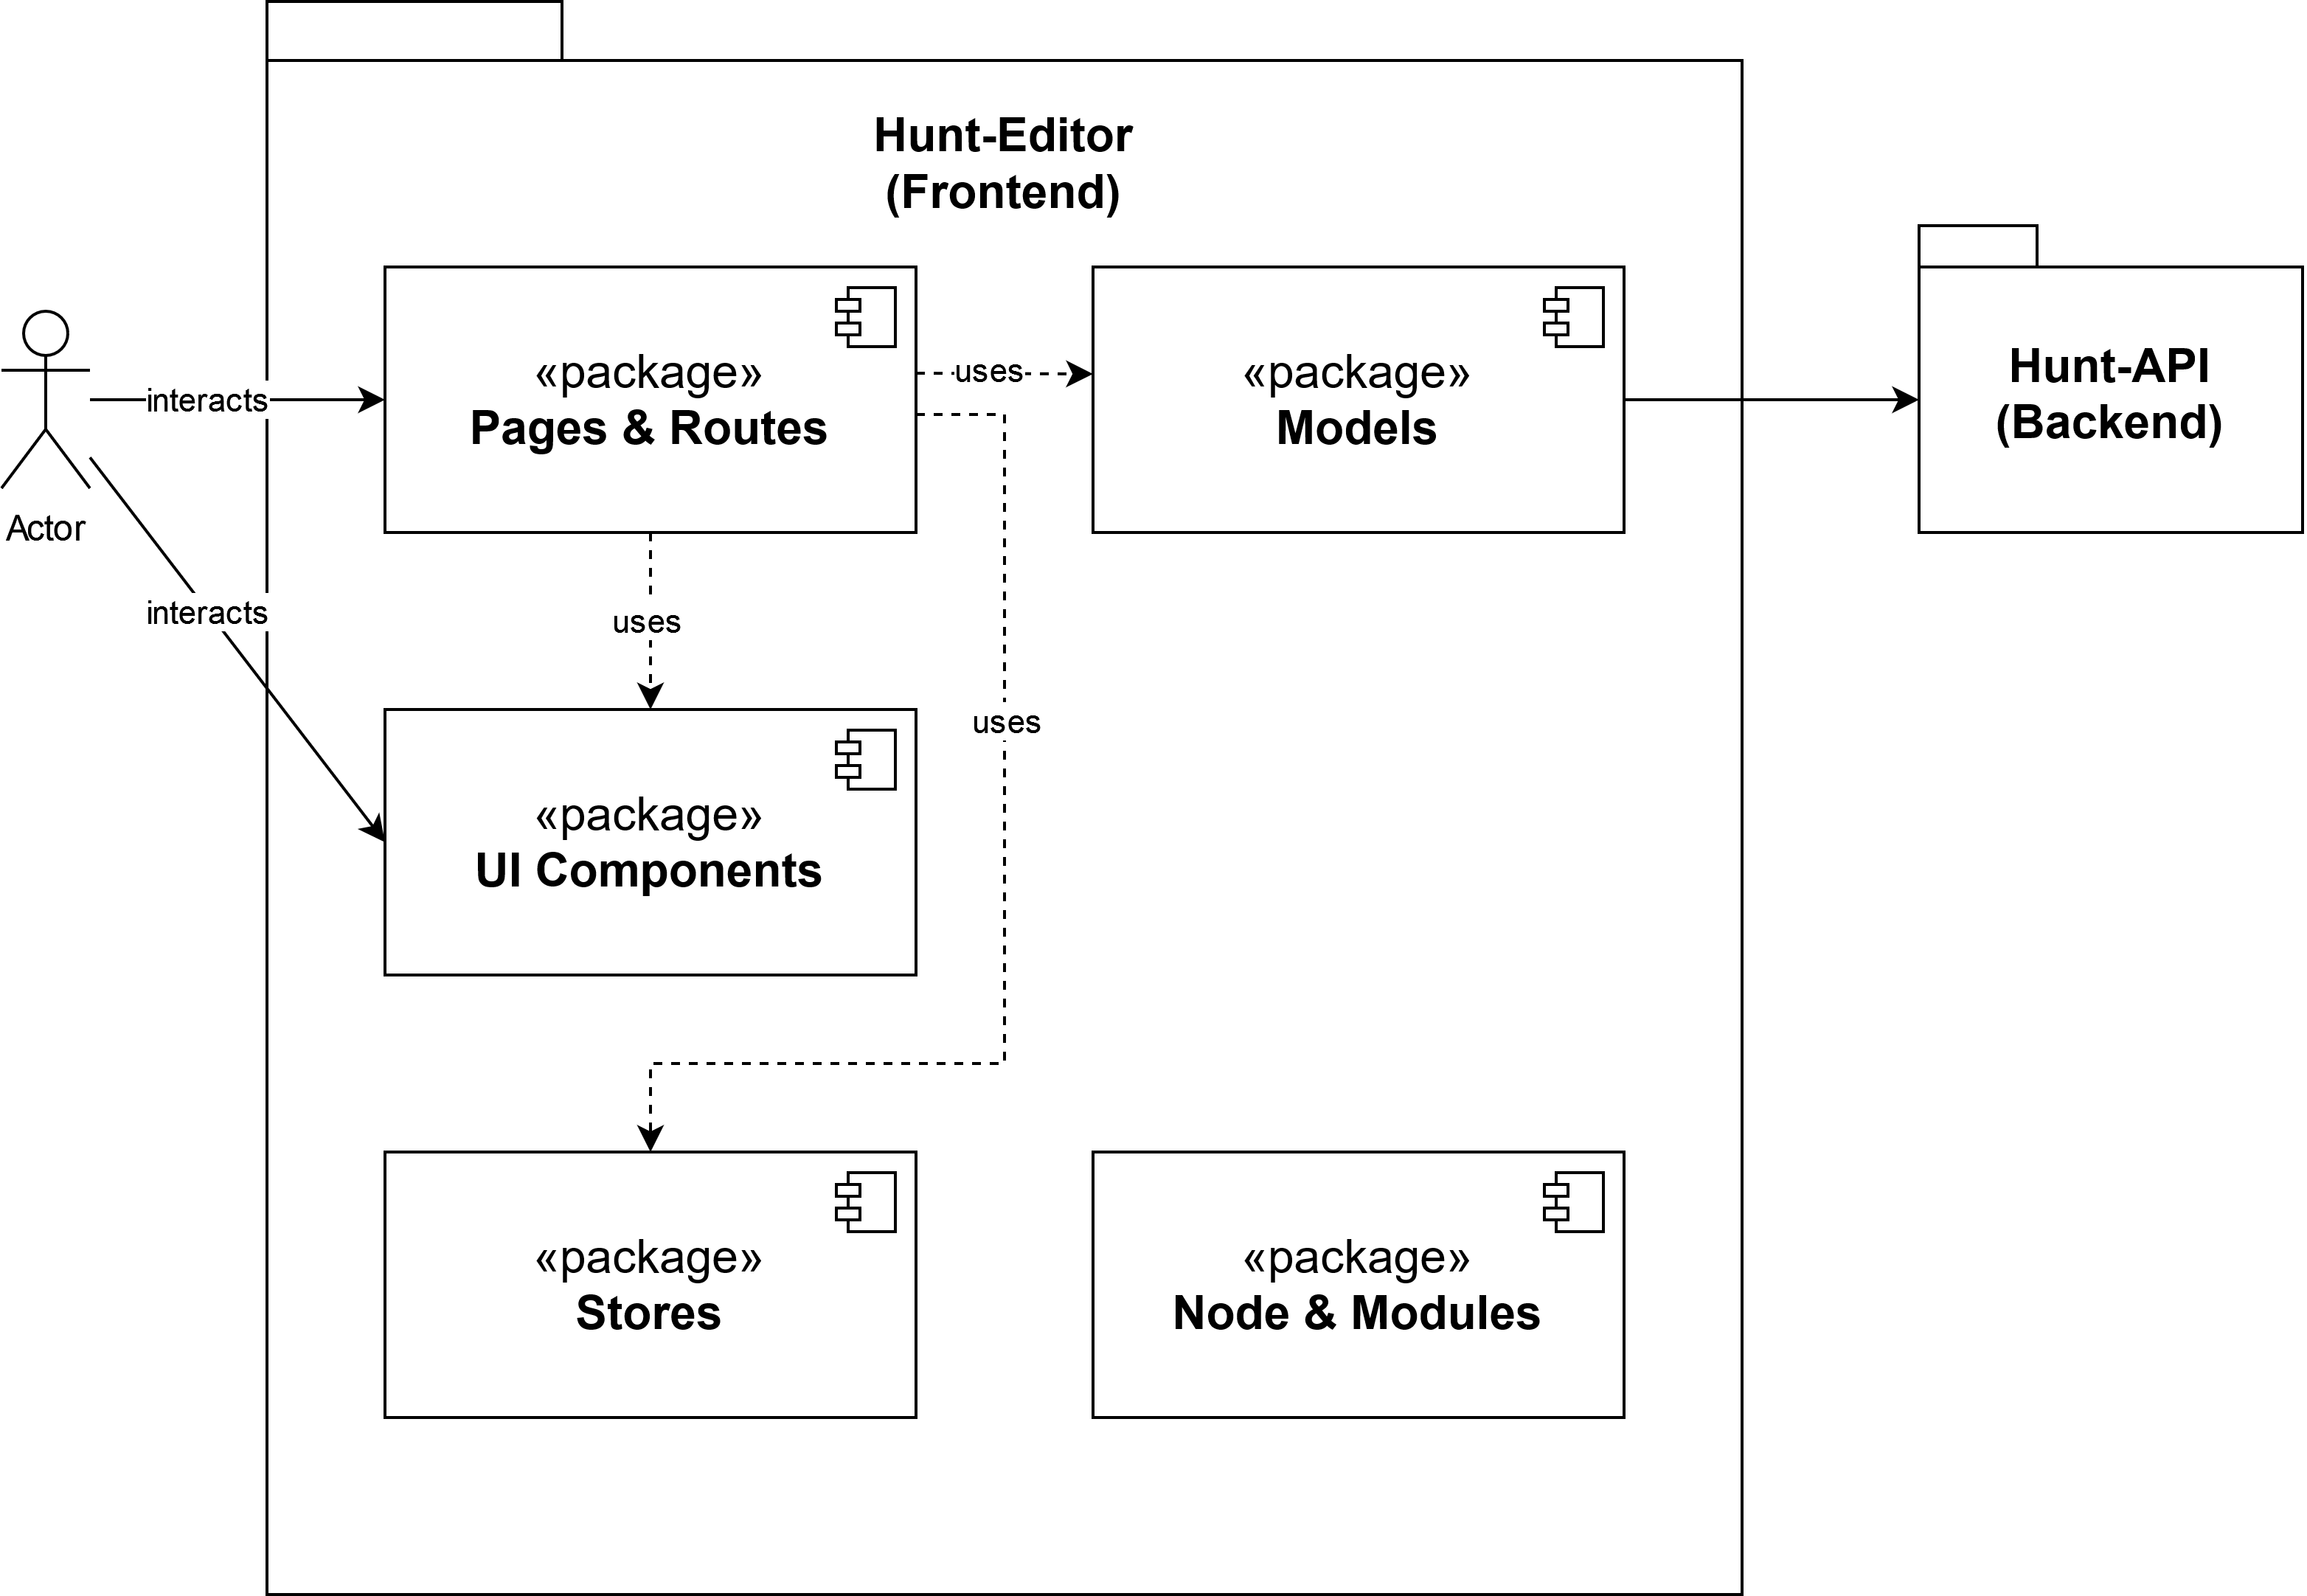
\includegraphics[width=1\textwidth]{images/PrAR-Loesung-Hunt-Editor-Components.png}
  \caption{UML-Diagramm Whitebox Frontend Hunt-Editor}
  \label{fig:whitebox-frontend}
\end{figure}

\textbf{Pages \& Routes}

Eine Svelte-Anwendung ist verzeichnisbasiert aufgebaut. Jedes Verzeichnis entspricht einer Route und kann ein oder mehrere Unterverzeichnisse haben, die die Route erweitern. Jede Route kann eine Seite haben, die immer den Namen \textit{+page.svelte} trägt. Svelte verwendet diese Seiten als Hauptanzeige, wenn zur zugehörigen Route navigiert wird.

Im Folgenden ist die Struktur des Routings als Baumdiagramm dargestellt.

\begin{figure}[H]
  \centering
  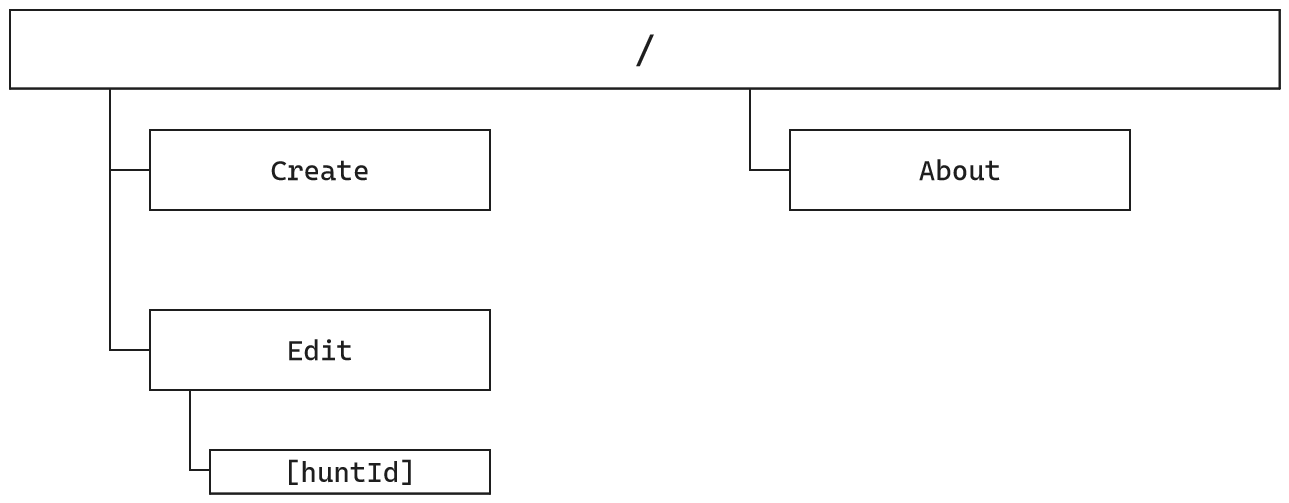
\includegraphics[width=1\textwidth]{images/PrAR-Loesung-Hunt-Editor-Routes.png}
  \caption{Skizze Frontend Hunt-Editor Routes}
  \label{fig:frontend-routes}
\end{figure}

Für die Anzeige und das Entfernen von Schnitzeljagden ist die Home Route \textit{/} vorgesehen. Auf der Route \textit{/about} werden Informationen zur Anwendung und zum Projekt bereitgestellt.

Der Workflow zum Erstellen einer Schnitzeljagd ist in der Route \textit{/create} implementiert.

Zum Editieren einer Schnitzeljagd werden die Komponenten aus der \textit{/create}-Route wiederverwendet, hier wird jedoch über die \textit{/edit/[huntId]}-Route gearbeitet, wobei \textit{[huntId]} ein Platzhalter für die \textit{Id} der jeweiligen Schnitzeljagd ist. Dadurch können dynamisch über die URL Informationen zur Schnitzeljagd abgerufen werden. Diese Informationen (wie bspw. Titel und Beschreibung) werden dann in die Eingabefelder eingetragen. 

\textbf{UI Components}

Für die Darstellung, Wiederverwendbarkeit und Konsistenz über verschiedene Seiten hinweg werden Svelte-Komponenten verwendet. Diese Komponenten bilden die Bausteine zur Anzeige unterschiedlicher Daten. Zusätzlich wurde die UI Component Library \textit{flowbite-svelte} verwendet, um standardisierte und ansprechende Benutzeroberflächenelemente wie Buttons, Inputs, Tabellen und andere UI-Komponenten effizient zu implementieren. Diese Bibliothek erleichtert die Entwicklung und trägt dazu bei, eine einheitliche und intuitive Benutzererfahrung sicherzustellen.

Jede Svelte-Komponente besteht aus einem Skript-Teil und einem Design-/Style-Teil. Eine Komponente kann auch weitere Komponenten einbinden. In diesem Fall fungiert die übergeordnete Komponente als Elternteil (Parent), während die eingebundenen Komponenten als Kinder (Children) bezeichnet werden.

\textbf{Stores}

Um während des Erstellungs- und Bearbeitungsprozesses Daten zu speichern, wird ein Svelte Store verwendet. Dies ermöglicht es verschiedenen Komponenten, auf diese Daten zuzugreifen. Beispielsweise kann die Komponente um Basisdaten einzugeben auf Titel und Beschreibung zugreifen, während die Komponente zum Anlegen/Bearbeiten der Aufgaben auf die Aufgaben zugreift.

\textbf{Node \& Node Modules}

\textit{Node.js} ist eine JavaScript-Laufzeitumgebung, die serverseitige Anwendungen ermöglicht. Sie stellt über den Paketmanager "\textit{npm}" Werkzeuge zur Verwaltung und Bereitstellung von externen Paket-Abhängigkeiten sowie Entwickler-Tools bereit. Neben dem Betrieb eines Webservers ermöglicht \textit{Node.js} auch die serverseitige Verarbeitung von API-Anfragen und die Anbindung an Datenbanken.

Eine Übersicht der einzelnen Paketabhängigkeiten wird in Kapitel \ref{swentwurf:hunt-editor:dependencies} gegeben.

\subsubsection{Wireframing}
Um den Editor zu entwickeln, der das Anlegen und Verwalten von Schnitzeljagden ermöglicht, wurde zunächst der Ansatz des Wireframings verwendet. Wireframing ist eine wesentliche Phase im Designprozess, die es ermöglicht, die Struktur und Funktionalität einer Anwendung visuell darzustellen, bevor detaillierte Design- und Entwicklungsarbeiten beginnen. In dieser frühen Planungsphase wird ein einfaches, oft schematisches Layout der Benutzeroberfläche erstellt, das die Anordnung der verschiedenen Elemente wie Buttons, Menüs, und interaktiven Komponenten zeigt. 

Im Folgenden werden die verschiedenen Wireframes aufgezeigt und erläutert, wieso sie eine solide Grundlage für die weitere Entwicklung des Editors boten, welche Stärken sie in Bezug auf Benutzerfreundlichkeit und Funktionalität aufwiesen, und welche Schwächen oder Herausforderungen während der Umsetzung erkannt wurden, die in späteren Phasen berücksichtigt werden mussten.

\begin{figure}[H]
  \centering
  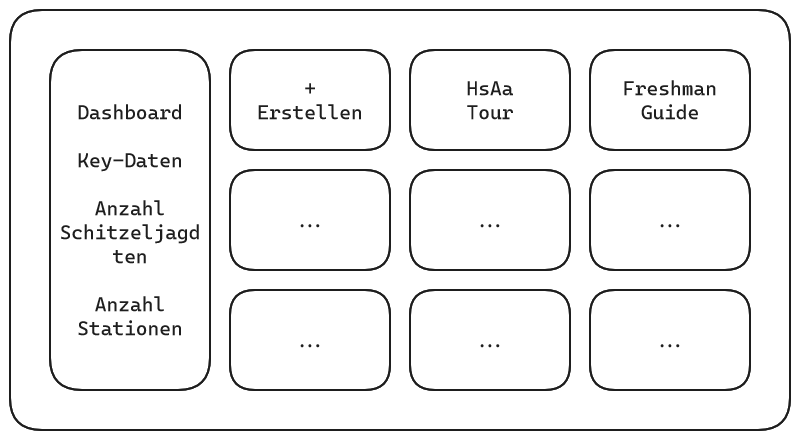
\includegraphics[width=1\textwidth]{images/wireframing/PrAr_Scavhunt_Wireframing-2.1.png}
  \caption{Wireframing Frontend Hunt-Editor 3}
  \label{fig:wireframing-frontend-hunt-editor-3}
\end{figure}

Dies war ein Wireframe, was relativ am Anfang der Entwicklungsphase entstanden ist. Hier wurde auf ein Grid-Layout gesetzt, um die Schnitzeljagden anzuzeigen. An der Seite befindet sich eine Sidebar, in der verschiedene Key-Daten abgelesen werden können. Da es aber durch Architekturänderungen keine Stationen mehr gibt, fällt diese Information weg. Das Grid-Layout sollte aber bestehen bleiben.

\begin{figure}[H]
  \centering
  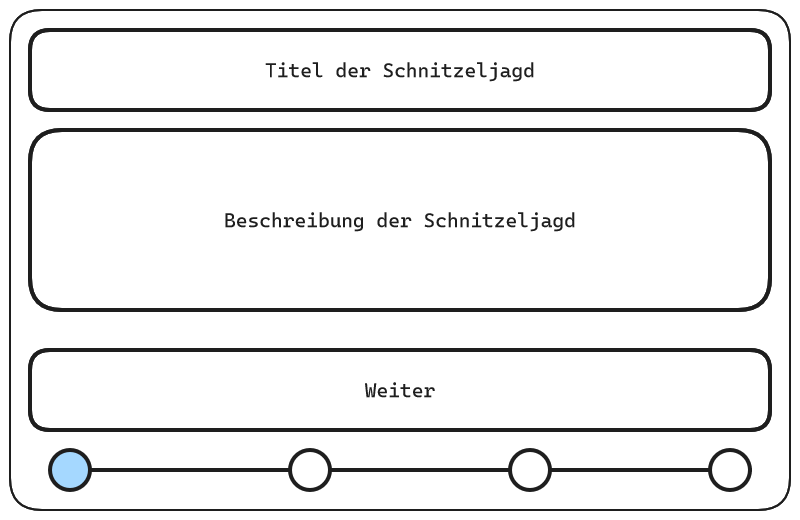
\includegraphics[width=1\textwidth]{images/wireframing/PrAr_Scavhunt_Wireframing-2.2.png}
  \caption{Wireframing Frontend Hunt-Editor 4}
  \label{fig:wireframing-frontend-hunt-editor-4}
\end{figure}

Hier wird nun der Prozess des Erstellen einer Schnitzeljagd beschrieben, gefallen hat uns hier das Verwenden einer Progressbar, um den aktuellen Fortschritt beim Erstellen anzuzeigen. Auch die Eingabe von Titel und Beschreibung sollte so später übernommen werden. 

\begin{figure}[H]
  \centering
  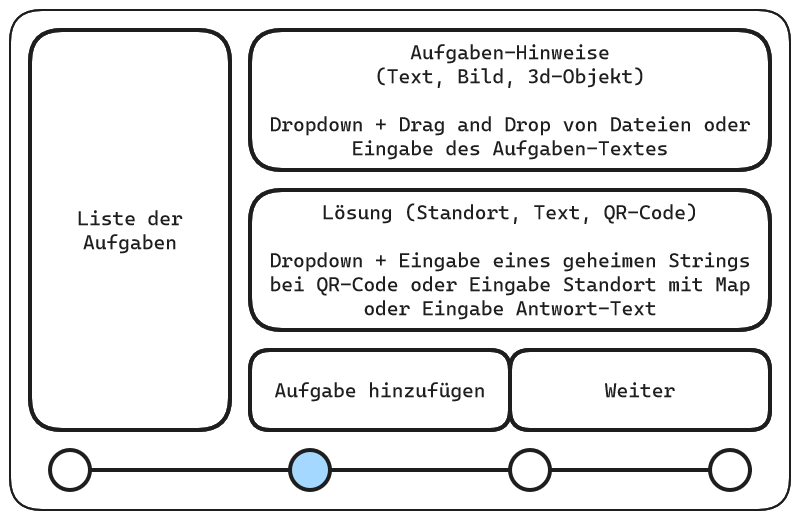
\includegraphics[width=1\textwidth]{images/wireframing/PrAr_Scavhunt_Wireframing-2.3.png}
  \caption{Wireframing Frontend Hunt-Editor 5}
  \label{fig:wireframing-frontend-hunt-editor-5}
\end{figure}

Nun zum schwersten Teil, das Anlegen und Bearbeiten von Aufgaben in einer Schnitzeljagd. Hier war zunächst der Ansatz, auf der linken Seite eine Tabelle der Aufgaben zu führen. Durch Klick auf die entsprechende Zeile werden dann auf der rechten Seite die Aufgabe und Lösung angezeigt. Hier ist auch noch der Aufgabentyp "3d-Objekt" vorhanden, welcher am Schluss nicht übernommen wurde. 

\begin{figure}[H]
  \centering
  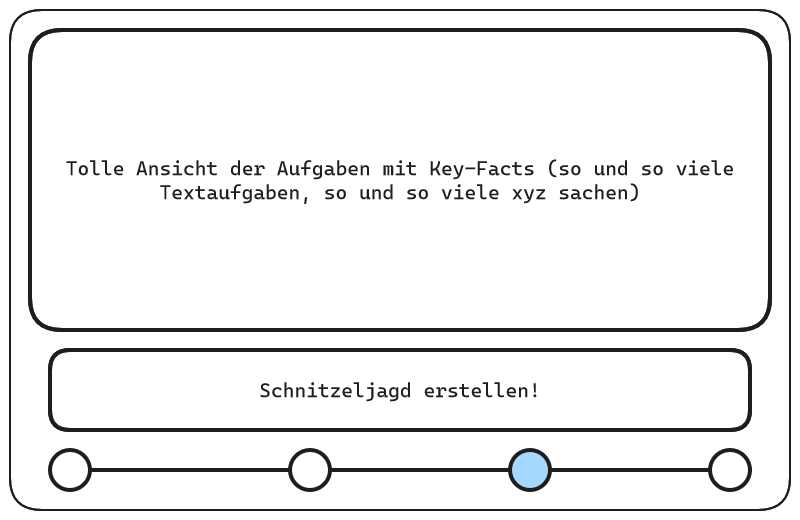
\includegraphics[width=1\textwidth]{images/wireframing/PrAr_Scavhunt_Wireframing-2.4.png}
  \caption{Wireframing Frontend Hunt-Editor 6}
  \label{fig:wireframing-frontend-hunt-editor-6}
\end{figure}

Dieses Wireframe zeigt zum Schluss nochmal eine Übersicht aller wichtigen Infos der Schnitzeljagd an. Dieses Konzept hat uns gut gefallen. 

\begin{figure}[H]
  \centering
  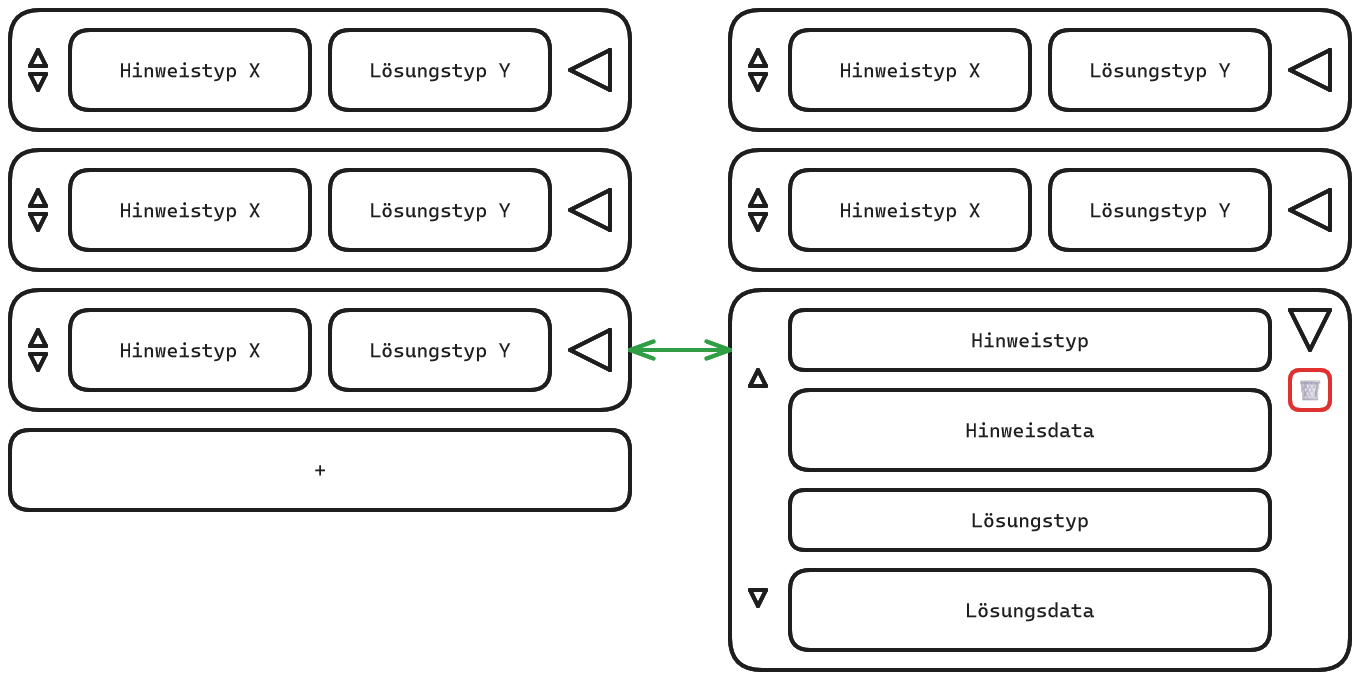
\includegraphics[width=1\textwidth]{images/wireframing/PrAr_Scavhunt_Wireframing-3.png}
  \caption{Wireframing Frontend Hunt-Editor 7}
  \label{fig:wireframing-frontend-hunt-editor-7}
\end{figure}

Da die seitliche Liste aus Abbildung \ref{fig:wireframing-frontend-hunt-editor-5} zum Anzeigen der Aufgaben für mobile Geräte ungeeignet ist, haben wir uns für den Ansatz aus Abbildung \ref{fig:wireframing-frontend-hunt-editor-7} entschieden. Hier werden die Aufgaben nacheinander angezeigt und deren Reihenfolgen kann über das Bedienen der Pfeiltasten angepasst werden. Um die Aufgaben zu bearbeiten, können diese über den Button auf der rechten Seite aufgeklappt und wieder zugeklappt werden. Im aufgeklappten Zustand befindet sich jeweils ein Dropdown für Aufgabe und Lösung als auch Eingabefelder / FileUpload oder eine Map Integration für Standort als Lösung. 

\subsubsection{Entscheidung Flowbite}
Um den Editor für das Verwalten von Schnitzeljagden zu erstellen, wurde zunächst versucht, mit DaisyUI zu arbeiten. Da dies nicht das gewünschte Ergebnis geliefert hat, wurde zu Flowbite gewechselt.

\paragraph{Unterschied zwischen Flowbite-Svelte und DaisyUI} \mbox{}\\
\textbf{DaisyUI} ist eine Komponentenbibliothek für Tailwind CSS, die eine Vielzahl von vorgefertigten UI-Komponenten bereitstellt. Es ist darauf ausgelegt, die Nutzung von Tailwind CSS zu vereinfachen, indem es gebrauchsfertige Klassen und Designs bietet. DaisyUI ist besonders bekannt für seine einfache Integration und die Möglichkeit, schnell und effizient ästhetisch ansprechende Benutzeroberflächen zu erstellen, ohne viel eigene CSS-Regeln schreiben zu müssen. 

Im Folgenden ein Beispiel für die Verwendung von DaisyUI, um ein Modal zu erstellen:

\begin{lstlisting}[language=html, caption={DaisyUI Beispiel}]
<button class="btn" onclick="my_modal_1.showModal()">open modal</button>
<dialog id="my_modal_1" class="modal">
  <div class="modal-box">
    <h3 class="text-lg font-bold">Hello!</h3>
    <p class="py-4">Press ESC key or click the button below to close</p>
    <div class="modal-action">
      <form method="dialog">
        <!-- if there is a button in form, it will close the modal -->
        <button class="btn">Close</button>
      </form>
    </div>
  </div>
</dialog>
\end{lstlisting}

\textbf{Flowbite-Svelte} ist eine auf Tailwind CSS basierende UI-Komponentenbibliothek, die speziell für die Integration mit Svelte entwickelt wurde. Sie bietet eine umfassende Sammlung von UI-Komponenten wie Buttons, Modale, Formulare und vieles mehr. Flowbite-Svelte kombiniert die Leistungsfähigkeit von Tailwind CSS mit der reaktiven Natur von Svelte, um die Entwicklung dynamischer und interaktiver Webanwendungen zu erleichtern. Zudem bietet Flowbite-Svelte eine nahtlose Svelte-Integration, was bedeutet, dass die Komponenten als echte Svelte-Komponenten bereitgestellt werden, die sich perfekt in das Svelte-Ökosystem einfügen. 

Im Folgenden ein Beispiel für die Verwendung von Flowbite-Svelte, das das gleiche Modal erstellt wie im DaisyUI-Beispiel:

\begin{lstlisting}[language=html, caption={Flowbite-Svelte Beispiel}]
<script>
  import { Button, Modal } from 'flowbite-svelte';
  let defaultModal = false;
</script>

<Button on:click={() => (defaultModal = true)}>open modal</Button>
<Modal title="Hello!" bind:open={defaultModal} autoclose>
  <p class="text-base leading-relaxed text-gray-500 dark:text-gray-400">Press ESC key or click the button below to close</p>
  <svelte:fragment slot="footer">
    <Button on:click={() => (defaultModal = false)}>Close</Button>
  </svelte:fragment>
</Modal>
\end{lstlisting}

\paragraph{Begründung für den Wechsel zu Flowbite-Svelte}\mbox{}\\
Der Wechsel von DaisyUI zu Flowbite-Svelte ist aus mehreren Gründen gerechtfertigt. Erstens bietet Flowbite-Svelte eine speziell auf Svelte abgestimmte Komponentenbibliothek, die eine engere und effizientere Integration ermöglicht. Dies bedeutet, dass die UI-Komponenten in Flowbite-Svelte als native Svelte-Komponenten verfügbar sind, was die Entwicklungsarbeit vereinfacht und die Nutzung von Svelte-spezifischen Features erleichtert.

Zweitens ist die Anpassungsfähigkeit und Erweiterbarkeit von Flowbite-Svelte ein wesentlicher Vorteil. Während DaisyUI zwar eine einfache Möglichkeit bietet, Tailwind CSS zu nutzen, ist Flowbite-Svelte besser darauf ausgelegt, komplexere und dynamischere Benutzeroberflächen zu unterstützen. Dies ist besonders wichtig für eine Anwendung wie den Schnitzeljagd-Editor, die eine hohe Interaktivität und eine benutzerfreundliche Oberfläche erfordert.

Darüber hinaus bietet Flowbite-Svelte eine breitere Palette an vorgefertigten Komponenten und Layout-Optionen, was die Entwicklung beschleunigt und gleichzeitig die Konsistenz und Qualität der Benutzeroberfläche verbessert. Dies trägt dazu bei, dass die Anwendung nicht nur funktional, sondern auch optisch ansprechend und intuitiv zu bedienen ist.

\subsubsection{Paketabhängigkeiten}
\label{swentwurf:hunt-editor:dependencies}

\begin{table}[H]
    \centering
    \begin{tabularx}{\textwidth}{|l|X|}
    \hline
    \textbf{Dependency} & \textbf{Beschreibung} \\
    \hline
    @sveltejs/adapter-auto & Adapter für SvelteKit, der automatisch den besten Adapter für die Zielumgebung auswählt \\
    \hline
    @sveltejs/kit & Das offizielle Framework zur Erstellung von Svelte-Anwendungen \\
    \hline
    @sveltejs/vite-plugin-svelte & Vite-Plugin zur Integration von Svelte \\
    \hline
    @types/eslint & TypeScript-Typdefinitionen für ESLint \\
    \hline
    @types/qrcode & TypeScript-Typdefinitionen für das qrcode-Paket \\
    \hline
    @types/uuid & TypeScript-Typdefinitionen für das uuid-Paket \\
    \hline
    autoprefixer & PostCSS-Plugin zur automatischen Ergänzung von Vendor-Präfixen in CSS \\
    \hline
    eslint & Ein pluggable Linter-Tool für JavaScript und JSX \\
    \hline
    eslint-config-prettier & ESLint-Konfiguration, die Konflikte zwischen ESLint und Prettier deaktiviert \\
    \hline
    eslint-plugin-svelte & ESLint-Plugin zur Unterstützung von Svelte \\
    \hline
    globals & Bibliothek, die globale Variablen und Umgebungen bereitstellt \\
    \hline
    postcss & Ein Werkzeug zur Transformation von CSS mit Plugins \\
    \hline
    prettier & Ein Code-Formatter, der konsistente Stilregeln erzwingt \\
    \hline
    prettier-plugin-svelte & Prettier-Plugin zur Formatierung von Svelte-Dateien \\
    \hline
    svelte & Das Svelte-Framework für reaktive Benutzeroberflächen \\
    \hline
    svelte-check & Ein Werkzeug zur statischen Analyse von Svelte-Projekten \\
    \hline
    tailwindcss & Ein Utility-First-CSS-Framework für die Erstellung maßgeschneiderter Designs \\
    \hline
    tslib & TypeScript-Hilfsbibliothek \\
    \hline
    typescript & Ein typisiertes Superset von JavaScript, das zu reinem JavaScript kompiliert \\
    \hline
    typescript-eslint & Eine Kombination von ESLint-Plugins und -Konfigurationen zur Unterstützung von TypeScript \\
    \hline
    vite & Ein schneller Entwicklungs-Server und Build-Tool, optimiert für moderne Webprojekte \\
    \hline
    
    \end{tabularx}
    \caption{Liste der verwendeten Dependencies und deren Beschreibung 1}
    \label{tab:dependencies-1}
\end{table}


\begin{table}[H]
    \centering
    \begin{tabularx}{\textwidth}{|l|X|}
    \hline
    \textbf{Dependency} & \textbf{Beschreibung} \\
    \hline
    @popperjs/core & Ein Tool zur Verwaltung von Popper-Elementen, wie Dropdowns und Tooltips \\
    \hline
    flowbite & Eine UI-Komponentenbibliothek basierend auf Tailwind CSS \\
    \hline
    flowbite-svelte & Eine Integration von Flowbite-Komponenten in Svelte \\
    \hline
    lucide-svelte & Eine Sammlung von Icons für Svelte \\
    \hline
    qrcode & Ein JavaScript-Toolkit zur Generierung von QR-Codes \\
    \hline
    tailwind-merge & Ein Utility zur Kombination und Zusammenführung von Tailwind CSS-Klassen \\
    \hline
    uuid & Ein Werkzeug zur Generierung von UUIDs (Universally Unique Identifiers) \\
    \hline
    \end{tabularx}
    \caption{Liste der verwendeten Dependencies und deren Beschreibung 2}
    \label{tab:dependencies-2}
\end{table}


\subsection{Participant Web-App}

\subsubsection{Übersicht}
% TODO 

\section{Architektonische Entscheidungen}

\subsection{Wahl eines Message-Bus für das Hunt-Api Backend}

% TODO: Beschreiben was für ein grund das hat, aka nicht valide teilnahmen erkennen.

\subsection{Wahl eines Api-Gateways für das Hunt-Api Backend}

% TODO: Beschreiben was das auf sich hat, aka nicht services einzelnd pingen aber einheitliche schnittstelle + eventuelle service sicherheit die später kommt durch sonder headers and stuff wenn wir das machen aber architektonisch einfach bessere wahl, ja der text macht grad wenig sinn weil ich aus irgwend nem grund irgendwas tippen will, bitte lächeln 

% AB HIER ARCHIVE
% AB HIER ARCHIVE
% AB HIER ARCHIVE
% AB HIER ARCHIVE

%\begin{figure}[H]
    %\centering
    %\includegraphics[width=\textwidth]{images/} TODO
    %\caption{Skizze der Systemarchitektur}
    % \label{fig:...} TODO
%\end{figure}

